\chapter{Definici\'on del modelo}
\label{sec-ca}
En esta secci\'on se concibe el modelo de aut\'omatas celulares que se presenta en este trabajo. Se comienza definiendo formalmente un aut\'omata celular~\cite[p\'agina 67]{book}.

\begin{definition}
\label{def-automata}
Un aut\'omata celular es una tupla $(\mathcal{L}; \mathcal{N}; \mathcal{E}; \mathcal{R})$ que se compone de los siguientes elementos representativos:
\begin{itemize}
\item [$\mathcal{L}$:] Es un conjunto potencialmente infinito de c\'elulas.
\item [$\mathcal{N}$:] $\mathcal{L} \times \mathcal{L} \rightarrow \lbrace 0,1 \rbrace$ es una funci\'on de vecindad, que puede ser vista como una relaci\'on, usualmente reflexiva y sim\'etrica, entre las c\'elulas. Esta funci\'on muestra qu\'e pares de c\'elulas son vecinas, o sea, la geometr\'ia de la organizaci\'on celular.
\item [$\mathcal{E}$:] Es un conjunto de estados. A cada c\'elula del conjunto $\mathcal{L}$ se le asigna un estado asociado en cada instante de tiempo.
\item [$\mathcal{R}$:] $\mathcal{E}^{|\mathcal{N}(v)|} \rightarrow \mathcal{E}$ es una funci\'on de transici\'on definida localmente. Esta funci\'on es el n\'ucleo de la din\'amica de un aut\'omata celular, y com\'unmente se expresa mediante reglas que definen el estado de la c\'elula en el siguiente instante de tiempo a partir del estado de las c\'elulas vecinas. El conjunto que contiene el estado de las c\'elulas vecinas se obtiene mediante la funci\'on $\mathcal{N}(v)$, que se define en~\ref{def-neighbourhood}.
\end{itemize}
\end{definition}

Un problema que surge al consultar la bibliograf\'ia sobre aut\'omatas celulares y modelos que hacen uso de los mismos es la notaci\'on y la formulaci\'on de los conceptos propios del tema. Diferentes autores proponen notaciones distintas para expresar ideas similares y definiciones generales que se adaptan a su problema particular, llevando a cabo una relajaci\'on del rigor matem\'atico. En el presente trabajo se utiliza la notaci\'on empleada en~\cite[p\'aginas 59-101]{book} escrita por Andreas Deutsch y Sabine Dormann, autores de numerosos art\'iculos relacionados con la modelaci\'on matem\'atica y, en especial, la modelaci\'on mediante aut\'omatas celulares.

\section{Hip\'otesis del modelo}
\label{subsec-hipo}
Como se expuso en la secci\'on~\ref{sec-cancer} el c\'ancer es una enfermedad extremadamente compleja compuesta por una gran cantidad de procesos, interacciones celulares y factores. Es parte del proceso de modelaci\'on lograr una simplificaci\'on del problema para hacerlo tratable, mediante la reducci\'on de la realidad a un conjunto de hip\'otesis. A continuaci\'on se plantean las hip\'otesis generales en las que se basa el presente modelo de aut\'omatas celulares, pero en secciones posteriores se expondr\'an suposiciones m\'as espec\'ificas a medida que se profundice en los distintos temas. El modelo toma como objeto de estudio al tipo de c\'ancer conocido como carcinoma o c\'ancer de c\'elulas epiteliales.

\begin{enumerate}
\item [{I.}] \textbf{Progresi\'on idealizada del desarrollo tumoral}: \emph{Se asume que el desarrollo tumoral sigue una progresi\'on idealizada dividida en las etapas avascular y vascular, donde el comportamiento macrosc\'opico del tumor est\'a definido por las mutaciones que expresan las c\'elulas cancer\'igenas.} \label{I}

\item [{II.}] \textbf{Mutaciones de las c\'elulas cancer\'igenas}: \emph{Se asume que la acumulaci\'on de mutaciones en la c\'elula cancer\'igena se define como un proceso secuencial y sigue un orden establecido, es decir, durante la etapa avascular se expresan las mutaciones relacionadas con el ciclo celular y la proliferaci\'on tumoral, y durante la etapa vascular se expresan las mutaciones relacionadas con la angiog\'enesis y met\'astasis, en adici\'on a las anteriores.} \label{II}

\item [{III.}] \textbf{Entidades biol\'ogicas del modelo}: \emph{Las entidades biol\'ogicas presentes en el modelo se componen \'unicamente de los tipos de c\'elulas definidos en el conjunto de estados del aut\'omata celular.} \label{III}

\item [{IV.}] \textbf{Interacciones entre las entidades del modelo}: \emph{Las interacciones entre las distintas c\'elulas del modelo se compone solamente por las reglas definidas en la funci\'on de transici\'on del aut\'omata.} \label{IV}

\item [{V.}] \textbf{Invarianza de las c\'elulas normales}: \emph{Se asume que la poblaci\'on de c\'elulas normales del organismo es est\'atica e invariante durante el transcurso del tiempo, es decir, no incurren en los procesos de divisi\'on ni muerte celular.} \label{V}

\item [{VI.}] \textbf{Homogeneidad de las c\'elulas cancer\'igenas}: \emph{Se asume que la poblaci\'on de c\'elulas cancer\'igenas que conforma la masa de un tumor es homog\'enea, es decir, no existen subtipos con mutaciones distintas o que est\'en en distintas etapas del ciclo celular.} \label{VI}

\item [{VII.}] \textbf{Suficiencia de nutrientes}: \emph{Se asume que el suministro de nutrientes y ox\'igeno es constante y suficiente para que todo tumor representado en el aut\'omata celular se desarrolle adecuadamente.} \label{VII}

\item [{VIII.}] \textbf{Desarrollo tumoral en funci\'on de la poblaci\'on}: \emph{Se asume que el avance de un tumor a trav\'es de las distintas etapas de su desarrollo depende \'unicamente de su poblaci\'on celular, descrita por la ecuaci\'on de Verhulst de crecimiento log\'istico.} \label{VIII}

\item [{IX.}] \textbf{Proceso de crecimiento simple}: \emph{El desarrollo tumoral se representa mediante un proceso de crecimiento simple, es decir, una posici\'on ocupada por una de estas c\'elulas tumorales permanece ocupada en los restantes instantes de tiempo, salvo que la masa cancer\'igena a la que pertenecen sea eliminada de la simulaci\'on como ocurre con las met\'astasis. } \label{IX}

\item [{X.}] \textbf{Adhesi\'on celular}: \emph{Se asume que la adhesi\'on de las c\'elulas tumorales se mantiene en todo momento salvo en los desprendimientos de c\'elulas migratorias como parte de la cascada metast\'asica.} \label{X}

\item [{XI.}] \textbf{V\'ias de la met\'astasis}: \emph{Se consideran solamente la diseminaci\'on hem\'atica y linf\'atica como v\'ias de la met\'astasis.} \label{XI}

\item [{XII.}] \textbf{Representaci\'on del tejido}: \emph{Se asume que un tejido puede ser representado mediante una red de mundo peque\~no, generada a partir del modelo Watts-Strogatz donde las coordenadas de los v\'ertices poseen dos componentes $x,y \in \mathbb{N}$ que constituyen la localizaci\'on de la c\'elula en el plano correspondiente con un corte de dicho tejido.} \label{XII}
\end{enumerate}

Esta \'ultima hip\'otesis es la que permite asumir que las conexiones cortas representan el contacto f\'isico entre dos c\'elulas debido a su proximidad, y las conexiones largas representan la posibilidad de que dos c\'elulas sean capaces de interactuar dada su conexi\'on a trav\'es del sistema circulatorio o linf\'atico. Adem\'as, esta hip\'otesis expone que no ser\'an considerados otros tipos de enlaces o interacciones entre las c\'elulas, y simplifica el posicionamiento espacial de las c\'elulas a partir sus coordenadas. Estas ideas se exponen con mayor profundidad en la secci\'on siguiente.

\section{Funci\'on de vecindad}
\label{subsec-vec}
Las redes complejas pueden representar un amplio rango de sistemas tanto en la sociedad humana como en la naturaleza. Tradicionalmente estos sistemas han sido modelados como grafos aleatorios, pero actualmente se conoce que la topolog\'ia y evoluci\'on de redes reales son gobernadas por principios de organizaci\'on robustos~\cite{complexnetworks}. El presente trabajo explora el comportamiento de aut\'omatas celulares definidos sobre un tipo de red compleja: las redes de mundo peque\~no, con el objetivo de modelar los mecanismos de invasi\'on, migraci\'on y met\'astasis de un tumor, y comparar los datos obtenidos con resultados existentes en la literatura cient\'ifica.

Un tejido blando es conjunto de c\'elulas interconectadas. Estas conexiones pueden ser de dos tipos. El primer tipo existe cuando hay una cercan\'ia f\'isica, e.g. el contacto entre las membranas de dos c\'elulas distintas. El segundo tipo se manifiesta cuando entre dos c\'elulas no existe el contacto f\'isico, pero est\'an conectadas a trav\'es del sistema circulatorio por su cercan\'ia a capilares sangu\'ineos o vasos linf\'aticos. Este \'ultimo tipo de conexi\'on se aprecia en la figura~\ref{fig-circulatory}. Esta conexi\'on se interpreta como la capacidad de una c\'elula cancer\'igena de interactuar con su c\'elula vecina normal y esta interacci\'on, a su vez, se define como la acci\'on de desplazar a la c\'elula normal de su posici\'on, para ser ocupada por la c\'elula cancer\'igena mediante un proceso de migraci\'on o por su propia descendencia. Las posibles interacciones se pueden apreciar en la figura \ref{fig-invasion}~\cite{kansal}.

\begin{figure}[p]
\begin{center}
\scalebox{0.7}{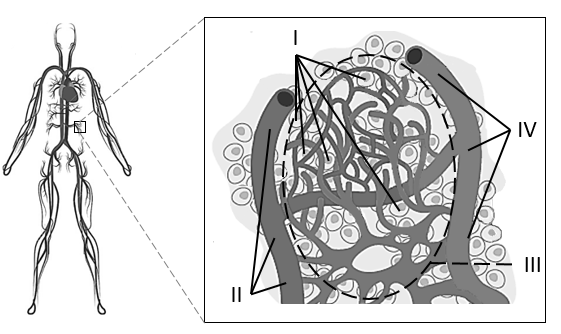
\includegraphics{img/circulatory-system.png}}
\end{center}\vspace*{-0.6cm}
\caption[Visualizaci\'on del sistema circulatorio en el organismo y de la circulaci\'on interna de un tejido]{Visualizaci\'on del sistema circulatorio en el organismo y de la circulaci\'on interna de un tejido. El sistema circulatorio es el encargado de conducir y circular la sangre por todo el organismo y la linfa unidireccionalmente hacia el coraz\'on. En la ampliaci\'on se aprecia el flujo de la circulaci\'on interna del tejido conformado por las c\'elulas~(\emph{I}) y sigue el siguiente recorrido: las arterias~(\emph{II}) traen la sangre oxigenada desde el coraz\'on, pasa por las arteriolas, capilares sangu\'ineos y v\'enulas~(\emph{III}) y finalmente desemboca en las venas~(\emph{IV}) que llevan la sangre de vuelta al coraz\'on para ser oxigenada nuevamente.}
\label{fig-circulatory}

\begin{center}
\scalebox{0.6}{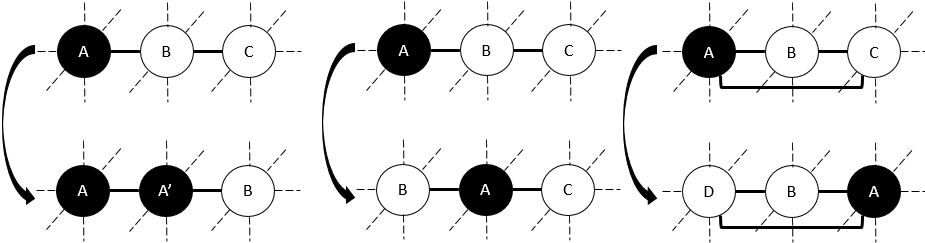
\includegraphics{img/fig-invasion.png}}
\end{center}\vspace*{-0.6cm}
\caption[Representaci\'on de las posibles interacciones entre c\'elulas cancer\'igenas y normales]{Representaci\'on de las posibles interacciones entre c\'elulas cancer\'igenas y normales.\newline
\textbf{Izquierda}: \textit{Divisi\'on Celular} - La c\'elula cancer\'igena A tiene una conexi\'on f\'isica con la c\'elula normal B. En el siguiente instante de tiempo, la c\'elula A se divide dando origen a la c\'elula cancer\'igena A' que pasa a ocupar la posici\'on de B, desplaz\'andola de la misma.\newline
\textbf{Centro}: \textit{Migraci\'on} - La c\'elula cancer\'igena A posee una mutaci\'on que le hace ganar movilidad y la posibilidad de migrar a trav\'es del tejido circundante, que le permite ocupar la posici\'on de la c\'elula normal B. En el siguiente instante de tiempo A se desplaza de su posici\'on, migra hacia B y la desplaza de su posici\'on, ocupando entonces la localizaci\'on de A.\newline
\textbf{Derecha}: \textit{Met\'astasis} - La c\'elula cancer\'igena A posee una conexi\'on distante con la c\'elula normal C, mediante su capacidad de penetrar el sistema circulatorio y abandonarlo en la posici\'on de C. En el siguiente instante de tiempo A se desplaza de su posici\'on, migra hacia C y la desplaza de su posici\'on. La localizaci\'on inicial de A es ocupada por una c\'elula normal D, descendiente de las c\'elulas vecinas de esa posici\'on.}
\label{fig-invasion}
\end{figure}

El conjunto de c\'elulas interconectadas se representa mediante una red, definida a partir de un grafo no dirigido con aristas entre vecinos inmediatos, correspondientes con el primer tipo de conexi\'on, y aristas entre v\'ertices distantes, correspondientes con el segundo tipo de conexi\'on.

\begin{definition}
\label{def-graph}
Sea $G(V, A)$ un grafo no dirigido donde los conjuntos $V$ y $A$ representan los v\'ertices y las aristas del grafo respectivamente. Se usa $V(G)$ y $A(G)$ para denotar los conjuntos de v\'ertices y aristas del grafo $G$ cuando dicho grafo no se enuncia en el contexto.
\end{definition}

\begin{definition}
\label{def-vertex-partition}
El conjunto de v\'ertices $V(G)$ est\'a dividido en dos subconjuntos $V_1(G)$ y $V_2(G)$ disjuntos que forman una partici\'on. Por tanto, satisfacen las siguientes propiedades: 
\begin{subequations}
\begin{equation}
V_1(G) \cup V_2(G) = V(G),
\end{equation}
\begin{equation}
V_1(G) \cap V_2(G) = \emptyset.
\end{equation}
\end{subequations}
\end{definition}

Los subconjuntos definidos en~\ref{def-vertex-partition} representan \'organos, tambi\'en llamadas localizaciones, que se corresponden con el \'organo primario donde se origina el c\'ancer y un \'organo preferencial de la met\'astasis, es decir, un \'organo que es colonizado con frecuencia por el tipo de c\'ancer que surgi\'o en el \'organo primario. Es necesario resaltar que ambas localizaciones pueden ser el mismo \'organo pero dos porciones distintas de tejido. Si se quiere indicar el subconjunto al que pertenece un v\'ertice $v$ determinado se utiliza la notaci\'on $V_v(G)$.

\begin{definition}
\label{def-edge-partition}
Los conjuntos $A^n(G)$ y $A^d(G)$ contienen las aristas del grafo que se corresponden con conexiones inmediatas y distantes respectivamente. Satisfacen las siguientes propiedades: 
\begin{subequations}
\begin{equation}
A^n(G) \cup A^d(G) = A(G),
\end{equation}
\begin{equation}
A^n(G) \cap A^d(G) = \emptyset.
\end{equation}
\end{subequations}
De esta manera estos subconjuntos de aristas constituyen una partici\'on del conjunto de aristas $A(G)$.
\end{definition}

A partir de los conjuntos $V(G)$ y $A(G)$ se definen los elementos representativos $\mathcal{L}$ y $\mathcal{N}$ del modelo de aut\'omatas celulares del presente trabajo de manera que se corresponda con lo expuesto en la definici\'on~\ref{def-automata}. Las declaraciones de los elementos representativos del aut\'omata celular aparecer\'an enmarcados en un recuadro negro para una mejor distinci\'on.

\begin{definition} 
\label{def-L}
El conjunto de c\'elulas $\mathcal{L}$ se define a partir del conjunto de v\'ertices del grafo $V(G)$ como se muestra a continuaci\'on: 
\begin{align}
\boxed{\mathcal{L} = V(G)}~. \label{eq-L}
\end{align}
\end{definition}

Con el objetivo de evitar ambig\"uedades y sin p\'erdida de rigor, cuando se vaya a referir al conjunto de c\'elulas siempre se utiliza el conjunto de v\'ertices $V(G)$. Los t\'erminos v\'ertice y c\'elula se utilizar\'an indistintamente. 

\begin{definition} 
\label{def-N}
La funci\'on de vecindad $\mathcal{N}$ se define a partir del conjunto de aristas del grafo $A(G)$ como se muestra a continuaci\'on:
\begin{subequations}
\begin{equation}
\boxed{\mathcal{N} : V(G) \times V(G) \rightarrow \lbrace 0,1 \rbrace}~, \label{eq-N}
\end{equation}
\begin{equation}
\boxed{\mathcal{N}(v,w) = \left\lbrace
	\begin{array}{lr}
		0& \textit{si } \lbrace v,w \rbrace \notin A(G)\\
		1& \textit{si } \lbrace v,w \rbrace \in A(G)
	\end{array}
\right.}~, \label{eq-N-2}
\end{equation}
\end{subequations}
o sea, los v\'ertices $v \in V(G)$ y $w \in V(G)$ son vecinos en el aut\'omata celular si existe una arista en $G$ que los conecta.
\end{definition}

\begin{definition}
\label{def-neighbourhood}
Se define a partir de la funci\'on de vecindad $\mathcal{N}(v,w)$ la vecindad del v\'ertice $v \in V(G)$ como el conjunto de v\'ertices $\mathcal{N}(v)$ que poseen aristas con el v\'ertice $v$, es decir:
\begin{align} 
\mathcal{N}(v) = \lbrace w~|~\mathcal{N}(v,w)=1 \rbrace. \label{eq-neighbourhood}
\end{align}
\end{definition}

\begin{definition}
\label{def-neighbourhoods}
Se define a partir del conjunto $\mathcal{N}(v)$ que contiene a los v\'ertices vecinos de $v$ los subconjuntos $\mathcal{N}^{n}(v) \subseteq \mathcal{N}(v)$ y $\mathcal{N}^{d}(v) \subseteq \mathcal{N}(v)$ que contienen los v\'ertices vecinos inmediatos y los v\'ertices vecinos distantes del v\'ertice $v$ respectivamente:
\begin{subequations}
\begin{equation}
\mathcal{N}^{n}(v) = \lbrace w~|~w \in \mathcal{N}(v) \wedge \lbrace v,w \rbrace \in A^n(G) \rbrace, \label{eq-neighbourhoods}
\end{equation}
\begin{equation}
\mathcal{N}^{d}(v) = \lbrace w~|~w \in \mathcal{N}(v) \wedge \lbrace v,w \rbrace \in A^d(G) \rbrace, \label{eq-neighbourhoods-2}
\end{equation}
\end{subequations}
\end{definition}

\section{Conjunto de c\'elulas: modelo Watts-Strogatz}
\label{subsec-watts}
En la secci\'on~\ref{subsec-vec} definimos un tejido blando como un conjunto de c\'elulas que presenta dos tipos de conexiones: entre c\'elulas vecinas cercanas y entre c\'elulas distantes. La generaci\'on de la red utilizada en el presente modelo de aut\'omatas celulares se expone a continuaci\'on. En~\cite{watts}, Duncan J. Watts y Steven H. Strogatz mostraron que existen muchas redes biol\'ogicas, tecnol\'ogicas y sociales que yacen entre las redes regulares y las aleatorias que tradicionalmente han sido utilizadas para modelar distintos tipos de sistemas din\'amicos. La clasificaci\'on y diferenciaci\'on de estas redes se lleva a cabo mediante los valores del coeficiente de agrupamiento~(\emph{clustering coefficient}) y la longitud promedio del camino~(\emph{average path length}). 

\begin{definition} 
\label{def-clustering}
Sea $v$ un v\'ertice del grafo que posee $k_v$ aristas que lo conectan a $k_v$ v\'ertices. El valor entre el n\'umero de aristas $K_v$ que existen en realidad entre estos $k_v$ v\'ertices y el n\'umero m\'aximo de aristas posibles\footnote{El n\'umero m\'aximo de aristas posibles se alcanza cuando los $k_v$ vecinos del v\'ertice $v$ pertenecen a un clique. Un clique en un grafo no dirigido es un conjunto de v\'ertices tal que para todo par de v\'ertices, existe una arista que los conecta.} $k_v(k_v-1)/2$ es el coeficiente de agrupamiento del v\'ertice $v$ y se determina como:
\begin{align}
C_v = \displaystyle\frac{2K_v}{k_v(k_v-1)}. \label{eq-clustering}
\end{align}
\end{definition}

\begin{definition}
\label{def-global-clustering}
El coeficiente de agrupamiento global del grafo $C_G$ es el promedio de todos los coeficientes de agrupamiento individuales $C_v$, es decir:
\begin{align}
C_G = \displaystyle\frac{1}{|V(G)|}\sum _{v=1} ^{|V(G)|} C_v. \label{eq-global-clustering}
\end{align}
\end{definition}

Si observamos la figura~\ref{fig-circulatory} las c\'elulas pertenecientes al tejido est\'an conectadas con numerosas c\'elulas vecinas inmediatas, y estas vecinas inmediatas est\'an conectadas entre s\'i. Dada la expresi\'on con que se determina el coeficiente de agrupamiento~(\ref{eq-clustering}) y la alta interconectividad existente se puede afirmar que la gran mayor\'ia de las c\'elulas pertenecientes al tejido poseen un alto coeficiente de agrupamiento. Por tanto, el coeficiente de agrupamiento global~(\ref{eq-global-clustering}) de la red tambi\'en posee un valor alto. 

En un grafo, la distancia entre dos v\'ertices es el menor n\'umero de aristas de un camino entre ellos. La longitud promedio del camino es la media de las distancias entre todo par de v\'ertices pertenecientes al grafo y se denota como $\ell_G$. La existencia de las numerosas conexiones distantes a trav\'es del sistema circulatorio hacen posible que el tejido posea un valor peque\~no de distancia para cualquier par de c\'elulas, ya que pueden estar conectadas mediante un camino que use estas conexiones. Podemos deducir entonces que esta red de c\'elulas posee una longitud promedio del camino relativamente peque\~na.

Como resultado podemos tomar como hip\'otesis que un tejido vivo posee un alto coeficiente de agrupamiento y una longitud promedio del camino peque\~na. Un tipo de red compleja que posee las caracter\'isticas anteriores son las redes de mundo peque\~no por lo que pueden ser utilizadas para representar un tejido vivo. Es posible generar grafos con estas caracter\'isticas usando el modelo de Watts y Strogatz~\cite{watts}. Los autores proponen un modelo de un solo par\'ametro que devuelve una red de mundo peque\~no, ubicada entre un grafo regular y un grafo aleatorio. El algoritmo propuesto por el modelo, que es utilizado para generar las redes de mundo peque\~no usadas en el presente trabajo, es el siguiente~\cite{complexnetworks}:

\begin{enumerate}
\item [(1)] \emph{Inicio:} Comenzamos con un grafo con $q$ v\'ertices, e.g. un anillo o una malla, en los que cada v\'ertice est\'a conectado a $k$ vecinos inmediatos. 

\item [(2)] \emph{Aleatorizaci\'on:} Reconectamos de forma aleatoria cada arista del grafo con una probabilidad $p$ de tal forma que no existan aristas duplicadas ni bucles. Este procedimiento introduce $\frac{p\,*\,q\,*\,k}{2} $ aristas que conectan v\'ertices distantes. Mediante la variaci\'on de $p$, se puede observar la transici\'on entre el orden con $p = 0$ y un grafo totalmente aleatorio con $p = 1$~(Fig.~\ref{fig-relations}).
\end{enumerate}

\begin{figure}[!ht]
\begin{center}
\scalebox{0.6}{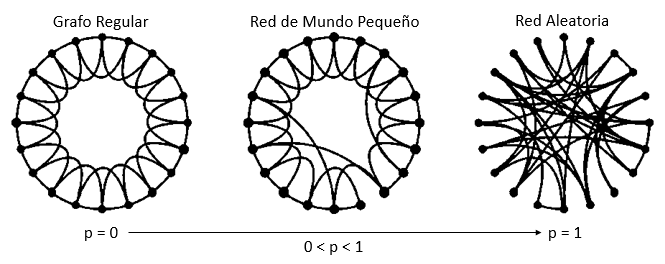
\includegraphics{img/fig-relations.png}}
\end{center}\vspace*{-0.6cm}
\caption[Proceso de reconexi\'on aleatoria del modelo Wattz-Strogatz]{Proceso de reconexi\'on aleatoria del modelo Wattz-Strogatz~(Figura tomada de~\cite{complexnetworks}). Se fijan $q = 20$ v\'ertices, cada uno conectado a sus cuatro vecinos m\'as cercanos. Para $p = 0$ el anillo original se queda inalterado, y a medida que se incrementa $p$ la red se vuelve desordenada. Para $p = 1$ todas las aristas del grafo son reconectadas.}
\label{fig-relations}
\end{figure}

\subsection{Implementaci\'on del modelo Watts-Strogatz}
\label{subsec-watts-2}
El modelo Watts-Strogatz, tomando en cuenta la hip\'otesis XII sobre la representaci\'on del tejido, parte de un grafo en el que cada v\'ertice ha sido conectado con un n\'umero de sus vecinos inmediatos. Las aristas que conforman el grafo son sometidas a un proceso de reconexi\'on, donde se modifica uno de los extremos de la arista. El nuevo extremo se elige de entre los v\'ertices restantes del grafo de forma aleatoria. Para el proceso de construcci\'on consideremos una cuadr\'icula que divide el plano en secciones iguales, donde cada celda se corresponde con un v\'ertice del grafo~(Fig.~\ref{fig-grid-2D-initial}).

\begin{figure}[!ht]
\begin{center}
\scalebox{0.7}{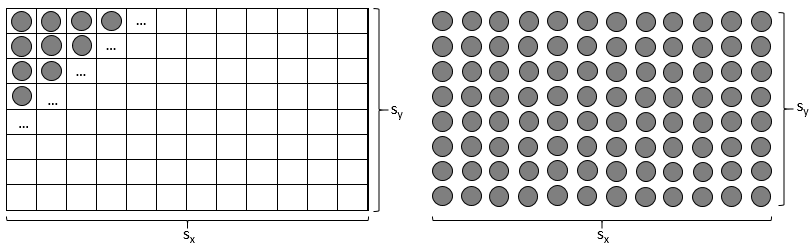
\includegraphics{img/fig-grid-2D-initial.png}}
\end{center}\vspace*{-0.6cm}
\caption[Disposici\'on espacial de los v\'ertices del grafo]{Disposici\'on espacial de los v\'ertices del grafo determinados mediante la cuadr\'icula que se muestra en la imagen izquierda, y que divide el plano en partes iguales para un total de $q = s_x \times s_y = 12 \times 8 = 96$ v\'ertices como se muestra en la imagen derecha.}
\label{fig-grid-2D-initial}
\end{figure}

Como se expuso en la definici\'on~\ref{def-neighbourhoods} el presente modelo de aut\'omatas celulares hace uso de los conjuntos $A^n(G)$ y $A^d(G)$ de aristas del grafo que se corresponden con conexiones inmediatas y distantes respectivamente. La idea de la implementaci\'on del modelo Watts-Strogatz para la construcci\'on del grafo es agregar todas las aristas inmediatas al conjunto $A^n(G)$ y a medida que sean reconectadas son removidas de este conjunto y se a\~naden a $A^d(G)$. Existen varias alternativas a la hora de elegir las conexiones inmediatas de cada v\'ertice donde cada una tiene un impacto importante sobre las propiedades de la red. En la figura~\ref{fig-neighbour} se pueden apreciar algunos diagramas de posibles configuraciones de vecindad. Comenzamos exponiendo la definici\'on de la distancia euclideana para definir posteriormente una funci\'on que permite obtener la vecindad inmediata de un v\'ertice. 

\begin{definition}
\label{def-euclidean-distance}
La funci\'on $d_E(v,w)$, que recibe dos v\'ertices $v \in V(G)$ y $w \in V(G)$, se corresponde con la distancia euclidiana entre los dos puntos del espacio que ocupan dichos v\'ertices y se determina como:
\begin{equation}
d_E(v,w)=\sqrt{(v_x-w_x)^2 + (v_y-w_y)^2}.
\end{equation}
\end{definition}

\begin{definition}
\label{def-neighbourhood-template}
Dado un v\'ertice $v$ en el sistema de coordenadas cartesianas que se utiliz\'o para crear la malla original, definimos como vecindad inmediata de $v$ al conjunto de v\'ertices $\mathcal{N}_I(v,R) = \lbrace w_1, w_2, \ldots, w_m \rbrace$ con $m=|\mathcal{N}_I(v,R)|$ que cumplen la condici\'on $d_E(v,w) \leq R$, es decir:
\begin{equation}
\mathcal{N}_I(v,R) = \lbrace w | d_E(v,w) \leq R \rbrace.
\end{equation}
\end{definition} 

\begin{figure}[!ht]
\begin{center}
\scalebox{0.5}{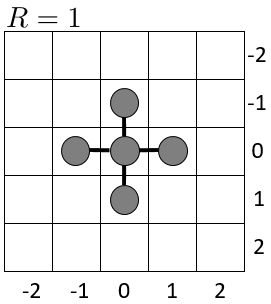
\includegraphics{img/fig-neighbour-R-1.png}}
\scalebox{0.5}{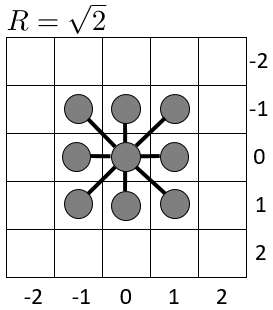
\includegraphics{img/fig-neighbour-R-sqrt(2).png}}
\scalebox{0.5}{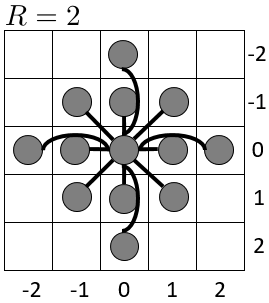
\includegraphics{img/fig-neighbour-R-2.png}}
\scalebox{0.5}{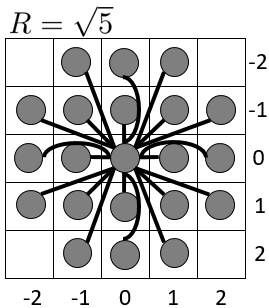
\includegraphics{img/fig-neighbour-R-sqrt(5).png}}
\end{center}\vspace*{-0.6cm}
\caption[Configuraciones de vecindad obtenidas mediante la variaci\'on de $R$]{Configuraciones de vecindad obtenidas mediante la variaci\'on de $R$. En todos los diagramas el v\'ertice $v=(0,0)$ es el centro de la configuraci\'on y se muestra en cada uno el valor de $R$ utilizado para generarla.}
\label{fig-neighbour}
\end{figure}

Es necesario tambi\'en discutir la inclusi\'on de aristas peri\'odicas al grafo. Una arista peri\'odica conecta dos extremos opuestos de la malla, por lo que la inclusi\'on de estas aristas constituye la implementaci\'on de una frontera peri\'odica en la malla. El modelo Watts-Strogatz asegura que el grafo creado posee las propiedades expuestas si todos los v\'ertices tienen el mismo grado, pero como se puede apreciar, un v\'ertice perteneciente a uno o varios lados del plano definido ser\'a referenciado por un n\'umero menor de aristas. La necesidad de incluir aristas peri\'odicas es una forma de hacer que estos v\'ertices posean el grado adecuado. La desventaja de este procedimiento es la ausencia de una interpretaci\'on natural de dichas aristas peri\'odicas por el modelo de aut\'omatas celulares que se presenta en este manuscrito. Se infiere que la inclusi\'on de estas aristas al grafo posee influencia sobre las propiedades del mismo. 

La selecci\'on de un valor adecuado de $R$, la probabilidad de reconexi\'on $p$ y la inclusi\'on de aristas peri\'odicas son los factores que determinan las propiedades del grafo resultante, cuestiones que se abordan en la secci\'on~\ref{subsec-R-periodic}. Finalmente, la implementaci\'on del modelo Watts-Strogatz se expone en el algoritmo~\ref{alg-watts} y los procedimientos que se llevan a cabo se detallan a continuaci\'on para mayor claridad.

\begin{algorithm}[!ht]
\caption{Implementaci\'on del Modelo Watts-Strogatz.} \label{alg-watts}
\KwData{$s_x, s_y, s_o, p, R$}
\KwResult{$G$}
$V_1=\lbrace \rbrace$\;
$V_2=\lbrace \rbrace$\;
$A^n=\lbrace \rbrace$\;
$A^d=\lbrace \rbrace$\;
\For{$i=0,1,\ldots,s_x-1$}{
	\For{$j=0,1,\ldots,s_y-1$}{
		$v=(i,j)$\;
		\eIf{$i < s_o$}{
			$V_1 = V_1 \cup v $\;}{
			$V_2 = V_2 \cup v $\;}}}
$V=V_1 \cup V_2$\;
\For{$v \in V$}{
	\For{$w \in N_I(v,R)$}{
		$a=\lbrace v,w \rbrace$\;
		$A^n=A^n \cup \lbrace a \rbrace$\;}}
\For{$\lbrace v,w \rbrace \in A^n$}{
	\If{$Random(0,1)<p$}{
		$A^n = A^n \setminus \lbrace v,w \rbrace$\;
		\Repeat{$\lbrace v,w' \rbrace \notin A^n \wedge \lbrace v,w' \rbrace \notin A^d \wedge v \neq w'$}
			{$w'=Select$-$Random$-$Vertex(V)$\;}
		$A^d = A^d \cup \lbrace v,w' \rbrace$\;}}
$A=A^n \cup A^d$\;
$G=(V,A)$\;
\Return $G$\;
\end{algorithm}

\paragraph{Declaraci\'on de los conjuntos que componen el grafo $G$ ($1$-$4$):} Se declaran los conjuntos $V_1$, $V_2$, $A_n$ y $A_d$, inicialmente vac\'ios, correspondientes con los v\'ertices de las localizaciones primaria y secundaria, y las conexiones inmediatas y distantes respectivamente. 

\paragraph{Crear v\'ertices ($5$-$11$):} Se a\~naden a los conjuntos $V_1$ y $V_2$ los v\'ertices que conforman el grafo. Cada v\'ertice $v$ de coordenadas $(v_x,v_y)$ se corresponde con una celda de la malla. Los valores $s_x$ y $s_y$ son las cantidades de v\'ertices del grafo por cada una de las componentes del plano respectivamente~(Fig.~\ref{fig-grid-2D-initial}). Cada v\'ertice se a\~nade al conjunto $V_1$ o $V_2$ correspondiente, que se determina a partir del par\'ametro $s_o$ con $0 \leq s_o < s_x$ que indica la divisi\'on del grafo entre una localizaci\'on y la otra. 

\paragraph{A\~nadir aristas inmediatas ($12$-$16$):} Se itera por todos los v\'ertices del grafo resultado de la uni\'on de los conjuntos $V_1$ y $V_2$. Por cada v\'ertice $v \in V$ se obtiene su vecindad inmediata $N_I(v,R)$ y se itera por todos los v\'ertices vecinos. Se crea una arista entre $v$ y cada v\'ertice vecino $w$ y se a\~nade al conjunto de aristas inmediatas $A^n$. Dado que la uni\'on entre conjuntos da como resultado un conjunto donde no existen elementos repetidos, no es necesario verificar si una nueva arista ya pertenece al conjunto $A^n$ antes de ser a\~nadida.

\paragraph{Reconexi\'on de las aristas ($17$-$26$):} Se itera por cada arista $a$ del grafo y con probabilidad $p$ se reconecta el v\'ertice destino de la arista. La generaci\'on del valor aleatorio que se compara con $p$ para el c\'alculo de la probabilidad sigue una distribuci\'on uniforme en $(0,1)$. La arista $\lbrace v,w \rbrace$ seleccionada para su reconexi\'on se elimina del conjunto $A^n$ y se procede a encontrar el nuevo v\'ertice destino. El nuevo v\'ertice destino $w'$ se elige de entre todos los v\'ertices del grafo, pero no puede ser el origen de la arista porque no se permiten bucles, y la nueva arista formada no puede existir en el grafo ya que no se permiten duplicados. La nueva arista $\lbrace v,w' \rbrace$ se a\~nade al conjunto $A^d$, identificando satisfactoriamente la nueva conexi\'on como distante. Finalmente, se realiza la uni\'on de los conjuntos $A^n$ y $A^d$, y se declara el grafo $G$ que se retorna como resultado del algoritmo. En la figura~\ref{fig-grid-2D-reconected} se puede apreciar la disposici\'on de los v\'ertices de las caras externas y las conexiones distantes una vez concluido el procedimiento.

\begin{figure}[!ht]
\begin{center}
\scalebox{0.65}{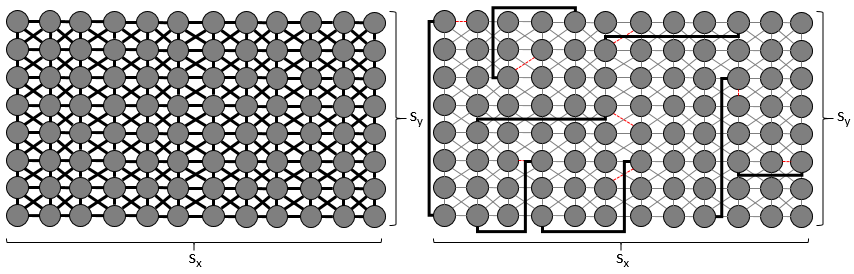
\includegraphics{img/fig-grid-2D-reconected.png}}
\end{center}\vspace*{-0.6cm}
\caption[Detalles de la disposici\'on de las aristas inmediatas y reconectadas en el grafo]{Detalles de la disposici\'on de las aristas inmediatas y reconectadas en el grafo presentado en la figura~\ref{fig-grid-2D-initial}. En el diagrama izquierdo se muestra el grafo construido utilizando la configuraci\'on de vecindad generada con $R=2$, y en el derecho se muestra el grafo una vez concluido el proceso de reconexi\'on de las aristas.}
\label{fig-grid-2D-reconected}
\end{figure}

\subsection{Propiedades del grafo resultante del modelo Watts-Strogatz}
\label{subsec-R-periodic}
En la secci\'on anterior se expuso que el valor del radio de la vecindad inmediata $R$ y las aristas peri\'odicas determinan las propiedades del grafo generado mediante el modelo Watts-Strogatz. Se propone en esta secci\'on exponer estad\'isticamente la medida en que afecta el coeficiente de agrupamiento global de la red y la longitud promedio del camino la ausencia o presencia de estas aristas en conjunci\'on con varios valores de $R$. Con el objetivo de efectuar esta prueba el algoritmo~\ref{alg-watts} puede alternar entre la inclusi\'on o no de las aristas peri\'odicas. Si se toma que la distancia euclideana entre dos v\'ertices que se encuentran en extremos opuestos del grafo $v$ y $w$ es igual a $1$~(siendo $R=1$ el menor valor de radio de la vecindad concebido) entonces la arista peri\'odica entre $v$ y $w$ estar\'a contenida en las vecindades inmediatas de estos v\'ertices. La implementaci\'on de esta condici\'on permite alternar entre la inclusi\'on o no de aristas peri\'odicas al grafo resultante.

Para verificar el impacto de las distintas configuraciones de vecindad inmediatas y de la inclusi\'on o no de aristas peri\'odicas en los valores del coeficiente de agrupamiento $C_G$ y de la longitud promedio del camino de la red $\ell_G$ se realizaron diversas pruebas mediante la construcci\'on de distintas redes con una cantidad total de $q = s_x \times s_y = 40 \times 20 = 800$ v\'ertices y alternando distintos valores de $R$ y $p$ con la inclusi\'on o no de aristas peri\'odicas. Cada uno de los valores de $C_G$ y $\ell_G$, mostrados en el cuadro~\ref{table-network-data}, fueron obtenidos promediando los resultados provenientes de la realizaci\'on de $30$ ejecuciones. 
\begin{table}[!ht]
\begin{center}
\scalebox{0.9}{\begin{tabular}{|c|c|c|c|c|c|c|c|c|} \hline
\multicolumn{3}{|c|}{\emph{Par\'ametros}} & \multicolumn{6}{|c|}{\emph{Probabilidad de reconexi\'on}} \\\cline{4-9}

\multicolumn{3}{|c|}{} & \multicolumn{1}{|l|}{$p=0~~$} & \multicolumn{1}{|l|}{$p=10^{-4}$} & \multicolumn{1}{|l|}{$p=10^{-3}$} & \multicolumn{1}{|l|}{$p=10^{-2}$} & \multicolumn{1}{|l|}{$p=10^{-1}$} & \multicolumn{1}{|l|}{$p=1~~$} \\\hline

 & \emph{Aristas} & $C_G$ & \multicolumn{1}{|r|}{$0$} & \multicolumn{1}{|r|}{$0$} & \multicolumn{1}{|r|}{$0$.$0001$} & \multicolumn{1}{|r|}{$0$.$0001$} & \multicolumn{1}{|r|}{$0$.$0007$} & \multicolumn{1}{|r|}{$0$.$0007$} \\\cline{3-9}
 
$R=1$ & \emph{peri\'odicas} & $\ell_G$ & \multicolumn{1}{|r|}{$15$} & \multicolumn{1}{|r|}{$14$.$9699$} & \multicolumn{1}{|r|}{$14$.$1113$} & \multicolumn{1}{|r|}{$10$.$2807$} & \multicolumn{1}{|r|}{$6$.$6847$} & \multicolumn{1}{|r|}{$5$.$1387$} \\\cline{2-9}

 & \emph{No aristas} & $C_G$ & \multicolumn{1}{|r|}{$0$} & \multicolumn{1}{|r|}{$0$} & \multicolumn{1}{|r|}{$0$} & \multicolumn{1}{|r|}{$0$} & \multicolumn{1}{|r|}{$0$.$0007$} & \multicolumn{1}{|r|}{$0$.$0042$} \\\cline{3-9}
 
 & \emph{peri\'odicas} & $\ell_G$ & \multicolumn{1}{|r|}{$19$.$975$} & \multicolumn{1}{|r|}{$19$.$8841$} & \multicolumn{1}{|r|}{$17$.$0731$} & \multicolumn{1}{|r|}{$11$.$8948$} & \multicolumn{1}{|r|}{$7$.$0317$} & \multicolumn{1}{|r|}{$5$.$2847$} \\\hline

 & \emph{Aristas} & $C_G$ & \multicolumn{1}{|r|}{$0$.$4284$} & \multicolumn{1}{|r|}{$0$.$4283$} & \multicolumn{1}{|r|}{$0$.$4271$} & \multicolumn{1}{|r|}{$0$.$4151$} & \multicolumn{1}{|r|}{$0$.$3155$} & \multicolumn{1}{|r|}{$0$.$0088$} \\\cline{3-9}
 
$R=\sqrt{2}$ & \emph{peri\'odicas} & $\ell_G$ & \multicolumn{1}{|r|}{$10$.$8165$} & \multicolumn{1}{|r|}{$10$.$6258$} & \multicolumn{1}{|r|}{$9$.$2563$} & \multicolumn{1}{|r|}{$6$.$6914$} & \multicolumn{1}{|r|}{$4$.$4453$} & \multicolumn{1}{|r|}{$3$.$4615$} \\\cline{2-9}

 & \emph{No aristas} & $C_G$ & \multicolumn{1}{|r|}{$0$.$4554$} & \multicolumn{1}{|r|}{$0$.$4554$} & \multicolumn{1}{|r|}{$0$.$4538$} & \multicolumn{1}{|r|}{$0$.$4423$} & \multicolumn{1}{|r|}{$0$.$3334$} & \multicolumn{1}{|r|}{$0$.$0089$} \\\cline{3-9}

 & \emph{peri\'odicas} & $\ell_G$ & \multicolumn{1}{|r|}{$14$.$8229$} & \multicolumn{1}{|r|}{$14$.$664$} & \multicolumn{1}{|r|}{$11$.$3451$} & \multicolumn{1}{|r|}{$7$.$5682$} & \multicolumn{1}{|r|}{$4$.$6398$} & \multicolumn{1}{|r|}{$3$.$5439$} \\\hline
    
 & \emph{Aristas} & $C_G$ & \multicolumn{1}{|r|}{$0$.$4328$} & \multicolumn{1}{|r|}{$0$.$4326$} & \multicolumn{1}{|r|}{$0$.$4228$} & \multicolumn{1}{|r|}{$0$.$4209$} & \multicolumn{1}{|r|}{$0$.$3219$} & \multicolumn{1}{|r|}{$0$.$0137$} \\\cline{3-9}
 
$R=2$ & \emph{peri\'odicas} & $\ell_G$ & \multicolumn{1}{|r|}{$7$.$6976$} & \multicolumn{1}{|r|}{$7$.$4887$} & \multicolumn{1}{|r|}{$6$.$9479$} & \multicolumn{1}{|r|}{$5$.$1801$} & \multicolumn{1}{|r|}{$3$.$6611$} & \multicolumn{1}{|r|}{$2$.$9432$} \\\cline{2-9}

 & \emph{No aristas} & $C_G$ & \multicolumn{1}{|r|}{$0$.$4731$} & \multicolumn{1}{|r|}{$0$.$4729$} & \multicolumn{1}{|r|}{$0$.$4716$} & \multicolumn{1}{|r|}{$0$.$4595$} & \multicolumn{1}{|r|}{$0$.$3506$} & \multicolumn{1}{|r|}{$0$.$0126$} \\\cline{3-9}
 
 & \emph{peri\'odicas} & $\ell_G$ & \multicolumn{1}{|r|}{$10$.$2375$} & \multicolumn{1}{|r|}{$9$.$8962$} & \multicolumn{1}{|r|}{$8$.$5608$} & \multicolumn{1}{|r|}{$5$.$6387$} & \multicolumn{1}{|r|}{$3$.$8089$} & \multicolumn{1}{|r|}{$3$.$0155$} \\\hline

 & \emph{Aristas} & $C_G$ & \multicolumn{1}{|r|}{$0$.$5157$} & \multicolumn{1}{|r|}{$0$.$5155$} & \multicolumn{1}{|r|}{$0$.$5138$} & \multicolumn{1}{|r|}{$0$.$501$} & \multicolumn{1}{|r|}{$0$.$3832$} & \multicolumn{1}{|r|}{$0$.$0235$} \\\cline{3-9}
 
$R=\sqrt{5}$ & \emph{peri\'odicas} & $\ell_G$ & \multicolumn{1}{|r|}{$5$.$9356$} & \multicolumn{1}{|r|}{$5$.$7967$} & \multicolumn{1}{|r|}{$5$.$0588$} & \multicolumn{1}{|r|}{$3$.$9797$} & \multicolumn{1}{|r|}{$3$.$0175$} & \multicolumn{1}{|r|}{$2$.$5704$} \\\cline{2-9}

 & \emph{No aristas} & $C_G$ & \multicolumn{1}{|r|}{$0$.$5697$} & \multicolumn{1}{|r|}{$0$.$5696$} & \multicolumn{1}{|r|}{$0$.$5679$} & \multicolumn{1}{|r|}{$0$.$5526$} & \multicolumn{1}{|r|}{$0$.$4186$} & \multicolumn{1}{|r|}{$0$.$0217$} \\\cline{3-9}

 & \emph{peri\'odicas} & $\ell_G$ & \multicolumn{1}{|r|}{$7$.$9587$} & \multicolumn{1}{|r|}{$7$.$6352$} & \multicolumn{1}{|r|}{$6$.$1198$} & \multicolumn{1}{|r|}{$4$.$2943$} & \multicolumn{1}{|r|}{$3$.$1359$} & \multicolumn{1}{|r|}{$2$.$6226$} \\\hline
\end{tabular}}
\end{center}\vspace*{-0.6cm}
\caption[Datos de las pruebas realizadas para verificar el impacto de las distintas configuraciones de vecindad y de la inclusi\'on de aristas peri\'odicas en las propiedades del grafo]{Datos de las pruebas realizadas para verificar el impacto de las distintas configuraciones de vecindad y de la inclusi\'on de aristas peri\'odicas en los valores del coeficiente de agrupamiento $C_G$ y de la longitud promedio del camino de la red $\ell_G$. }
\label{table-network-data}
\end{table}

Se observa que para un mismo valor de $R$ e independientemente si se incluyen o no las aristas peri\'odicas, a medida que aumenta el valor de la probabilidad de reconexi\'on $p$ disminuye el coeficiente de agrupamiento global y disminuye la longitud promedio del camino, observ\'andose la mayor disminuci\'on a medida que $p$ se acerca a $1$. Esto ocurre porque a medida que m\'as aristas inmediatas son reconectadas a v\'ertices distantes es menor la probabilidad de que estos v\'ertices distantes est\'en conectados con los vecinos inmediatos del v\'ertice focal, disminuyendo el valor del coeficiente de agrupamiento del grafo; pero a medida que aparecen m\'as aristas distantes aumenta la probabilidad de que dos v\'ertices aleatorios est\'en conectados a trav\'es de un camino m\'as corto que utilice estas aristas, disminuyendo la longitud promedio del camino.

Adem\'as se cumple para toda combinaci\'on de $R$ y $p$ que la ausencia de aristas peri\'odicas en el grafo hace que la longitud promedio del camino aumente, dado que permiten la existencia de posibles caminos entre v\'ertices distantes que poseen distancias menores que los caminos que no cuentan con dichas aristas. Pero la ausencia de aristas peri\'odicas, salvo para $p=1$, provoca tambi\'en un aumento en el coeficiente de agrupamiento del grafo, dado que los v\'ertices que poseen vecinos conectados por aristas peri\'odicas aportan valores peque\~nos del coeficiente de agrupamiento ya que existen muchos casos donde dichos v\'ertices vecinos no est\'an conectados entre s\'i.

Dado que la presencia de aristas peri\'odicas carece de una interpretaci\'on natural como se mencion\'o en la secci\'on~\ref{subsec-watts-2}, y que no afectan de forma negativa las propiedades deseadas del grafo resultante como se expuso en el texto anterior, se decide no incluirlas. Se elige la configuraci\'on de vecindad generada con $R=\sqrt{2}$ ya que los grafos construidos con este valor poseen coeficientes de agrupamiento altos y longitudes promedio del camino relativamente peque\~nas. Adem\'as constituye la configuraci\'on de vecindad m\'as sencilla que posee las caracter\'isticas mencionadas ya que provee de una interpretaci\'on natural para las conexiones inmediatas correspondientes con la cercan\'ia f\'isica a diferencia de otras vecindades generadas con valores mayores de $R$; e.g. para $R=2$ se tienen v\'ertices vecinos a distancia $2$ del v\'ertice central. En cuanto a la probabilidad de reconexi\'on esta se encuentra entre los valores $p \in \lbrace 10^{-3}, 10^{-2} \rbrace$ en los que ocurre un r\'apido descenso en el valor de la longitud promedio del camino mientras que el coeficiente de agrupamiento se mantiene casi invariante con un valor cercano a $C_G=0$.$45$ para $R=\sqrt{2}$, que si atendemos lo planteado en~\cite{complexnetworks} constituye un valor alto.

\section{Conjunto de estados}
\label{subsec-states}
Un estado en teor\'ia de aut\'omatas celulares es un valor num\'erico que se le asigna inicialmente a cada elemento del conjunto de c\'elulas y puede cambiar en el transcurso de la ejecuci\'on. En este modelo el estado indica el tipo de c\'elula biol\'ogica en la que estamos en presencia. Un corte transversal del tejido revela que est\'a estructurado en capas donde cada una posee una funci\'on espec\'ifica dentro del \'organo~(Fig.~\ref{fig-structure}). El desarrollo macrosc\'opico de un tumor depende en gran medida de las interacciones progresivas entre la masa de las c\'elulas cancer\'igenas y cada una de estas capas de tejidos. En \'epocas pasadas de la histolog\'ia\footnote{La histolog\'ia es la disciplina que estudia todo lo relacionado con los tejidos org\'anicos: su estructura microsc\'opica, su desarrollo y sus funciones.} se clasificaba cada capa del tejido como parte del par\'enquima o del estroma. Se reconoce como par\'enquima al tejido que desempe\~na la funci\'on principal de un \'organo espec\'ifico, mientras que las capas de tejido que hacen de sost\'en y apoyo al tejido funcional se llama estroma. Generalmente el par\'enquima est\'a conformado por el epitelio de un \'organo. En la secci\'on~\ref{subsec-macro} se expuso el desarrollo idealizado de un tumor que se origina en c\'elulas de tipo epitelial o carcinoma, y su expansi\'on a trav\'es de las distintas capas de tejidos. Por lo que, en primera instancia, se requiere de un estado para las c\'elulas del tejido epitelial.

\begin{figure}[!ht]
\begin{center}
\scalebox{0.6}{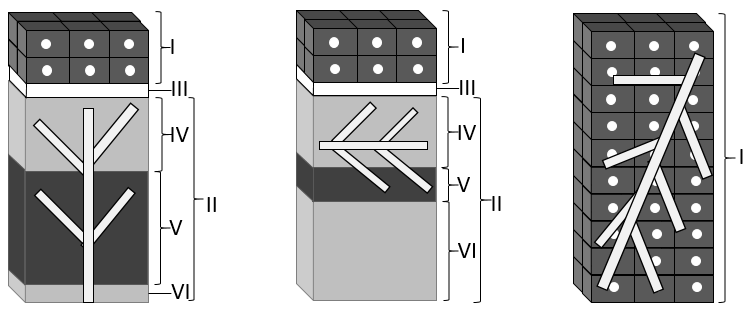
\includegraphics{img/fig-structure.png}}
\end{center}\vspace*{-0.6cm}
\caption[Distribuci\'on de las capas de tejidos en distintos \'organos]{Distribuci\'on de las capas de tejidos en distintos \'organos afectados com\'unmente por el tipo de c\'ancer conocido como carcinoma~\cite{robins}.\newline
\textbf{Izquierda}: \textit{Aparato digestivo} - La estructura mostrada est\'a presente en el es\'ofago, est\'omago, intestinos y recto~\cite{stomach}. Como se puede apreciar todos los tejidos de sost\'en presentan vasculatura. Todas las formas de carcinomas que afectan al aparato digestivo comienzan en la mucosa: carcinoma de c\'elulas escamosas del es\'ofago, adenocarcinoma g\'astrico y adenocarinoma colonrectal. La leyenda se muestra a continuaci\'on: mucosa~(\emph{I}) - formada por epitelio escamoso estratificado en el es\'ofago y por epitelio cil\'indrico columnar en est\'omago e intestinos; estroma~(\emph{II}) - tejidos de sost\'en; membrana basal~(\emph{III}); submucosa~(\emph{IV}) - formada por tejido conjuntivo; muscularis propia~(\emph{V}); serosa~(\emph{VI}).\newline
\textbf{Centro}: \textit{Pulm\'on} - La estructura mostrada est\'a presente en las v\'ias a\'ereas inferiores compuestas por tr\'aquea, bronquios y bronquiolos~\cite{lung}. Como se puede apreciar todos los tejidos de sost\'en con la excepci\'on del cart\'ilago hialino presentan vasculatura. El carcinoma pulmonar de c\'elulas escamosas comienza en la mucosa de los bronquios en la mayor\'ia de los casos. La leyenda se muestra a continuaci\'on: mucosa~(\emph{I}) - formada por epitelio pseudoestratificado columnar en la tr\'aquea y bronquios primarios y por epitelio simple cil\'indrico en los bronquiolos; estroma~(\emph{II}) - tejidos de sost\'en; membrana basal~(\emph{III}); submucosa~(\emph{IV}) - formada por tejido conjuntivo; m\'usculo liso~(\emph{V}); cart\'ilago hialino~(\emph{VI}) - formado por tejido conjuntivo duro.\newline
\textbf{Derecha}: \textit{H\'igado} - El h\'igado est\'a conformado por su propio tipo de c\'elula: los hepatocitos~(\emph{I}) y constituyen su par\'enquima~\cite{liver}. Los vasos del sistema circulatorio est\'an presentes a lo largo del \'organo. El c\'ancer de h\'igado que surge en esta clase de c\'elulas se considera como un carcinoma y se conoce como hepatocarcinoma, aunque las met\'astasis en el h\'igado de otros tipos de c\'ancer son mucho m\'as frecuentes que los que comienzan en el propio \'organo.}
\label{fig-structure}
\end{figure}

Se han hecho progresos en el entendimiento de las complejas interacciones entre el tumor y el tejido sano del organismo, en especial las responsables de los comportamientos invasivos y migratorios del c\'ancer, pero muchos mecanismos no son comprendidos en su totalidad o se desconocen por completo en este momento~\cite{kansal3}. Sin embargo se pueden distinguir varios procesos responsables de la invasi\'on y migraci\'on: la degradaci\'on de la membrana basal que se desarrolla durante la angiog\'enesis, la deformaci\'on y desplazamiento del estroma como consecuencia de las fuerzas generadas por la expansi\'on del tumor y la degradaci\'on de la ECM~\cite{kansal3}. El tipo de c\'elula cancer\'igena que entra en contacto con el estroma define cual proceso se llevar\'a a cabo. La invasi\'on se lleva a cabo por c\'elulas cancer\'igenas pertenecientes a la masa del tumor una vez que se ha degradado la membrana basal, y la migraci\'on por c\'elulas cancer\'igenas que poseen las mutaciones para desplazarse a trav\'es del estroma mediante la degradaci\'on de la ECM. 

A pesar de la heterogeneidad de los tejidos que conforman el estroma, las interacciones entre la totalidad de los tejidos de sost\'en y las c\'elulas cancer\'igenas resultan en uno de estos dos procesos: invasi\'on o migraci\'on. Por este motivo no es necesario distinguir entre las distintas capas de tejidos de sost\'en en el aut\'omata celular si solo se tienen en cuenta estas interacciones fundamentales. Luego se adopta una nueva hip\'otesis en el modelo que reduce la complejidad de la din\'amica del aut\'omata celular, representando los distintos tipos de tejidos de sost\'en simplemente como estroma. Las c\'elulas del aut\'omata correspondientes a este tejido se corresponden entonces a c\'elulas biol\'ogicas reales o a cl\'usteres de macromol\'eculas presentes en la ECM. 

\begin{itemize}
\item [{XIII.}] \textbf{Tejidos de sost\'en o estroma}: \emph{Se representa a la totalidad de los tejidos de sost\'en de un \'organo simplemente como estroma debido a que solo se consideran dos interacciones fundamentales entre los tejidos sanos y el c\'ancer: la invasi\'on y la migraci\'on. Por este motivo no es necesario hacer distinciones entre las distintas capas de sost\'en.} \label{XIII}
\end{itemize}

El tejido epitelial recubre toda superficie del cuerpo humano que tiene contacto con el exterior, e.g. \'organos huecos, como el est\'omago y pulmones, o estructuras tubulares, como los bronquios y arterias. Estos espacios se conocen como luz de un \'organo o lumen, en el caso de los bronquios, arterias e intestinos. En los carcinomas es com\'un que la masa tumoral brote fuera del epitelio, evadiendo los controles de homeostasis del tejido y volvi\'endose una lesi\'on. La manifestaci\'on fuera del epitelio constituye un marcador visible del desarrollo neopl\'asico, por lo que la luz de un \'organo o lumen debe ser representada~\cite{robins,stomach,lung,liver,breast}. A partir de lo expuesto anteriormente se infieren los estados para las c\'elulas normales. A continuaci\'on se define formalmente el estado de una c\'elula del aut\'omata:

\begin{definition}
\label{def-cellstatus}
Sea un v\'ertice $v \in V(G)$ y un instante de tiempo $n$ del aut\'omata. Se define entonces la funci\'on $s(v,n)$ que devuelve el estado del v\'ertice $v$ en el instante de tiempo $n$:
\begin{subequations}
\begin{equation}
s: V(G) \times \mathbb{N} \rightarrow \mathcal{E}, \label{eq-cellstatus}
\end{equation}
\begin{equation}
s(v,n) = e_i, \label{eq-cellstatus-2}
\end{equation}
\end{subequations}
donde $e_i$ es un estado cualquiera del conjunto de estados $\mathcal{E}$, es decir, $e_i \in \mathcal{E},~\forall i \in \lbrace 0, \ldots, |\mathcal{E}| \rbrace$.
\end{definition}

A continuaci\'on, tomando en cuenta la hip\'otesis XIII sobre los tejidos de sost\'en, se disponen los estados para las c\'elulas normales del aut\'omata:

\begin{itemize}
\item $s(v,n)=0$: El v\'ertice $v$ posee el estado correspondiente con el espacio vac\'io o lumen en el instante de tiempo $n$, y representa las cavidades huecas de los \'organos y conductos.

\item $s(v,n)=1$: El v\'ertice $v$ representa una c\'elula del epitelio en el instante de tiempo $n$, y corresponde con el tejido donde se origina el carcinoma.

\item $s(v,n)=2$: El v\'ertice $v$ posee el estado correspondiente con el estroma en el instante de tiempo $n$, y representa el conjunto de tejidos de sost\'en del \'organo.
\end{itemize}

En cuanto a las c\'elulas cancer\'igenas se distinguen tres estados fundamentales basado en las hip\'otesis del modelo y en lo expuesto en la secci\'on~\ref{sec-cancer}:

\begin{itemize}
\item $s(v,n)=3$: El v\'ertice $v$ representa una c\'elula tumoral en el instante de tiempo $n$, y constituyen la masa neopl\'asica.

\item $s(v,n)=4$: El v\'ertice $v$ representa una c\'elula migratoria en el instante de tiempo $n$, es decir, poseen las mutaciones necesarias para efectuar la cascada metast\'asica.

\item $s(v,n)=5$: El v\'ertice $v$ representa una c\'elula micrometast\'asica en el instante de tiempo $n$, es decir, efectuaron la cascada metast\'a\-sica satisfactoriamente y est\'an colonizando la nueva localizaci\'on, pero pueden ser destruidas por el sistema inmunitario o fallar en dicha colonizaci\'on. 
\end{itemize}

Luego el conjunto de estados tiene la forma:
\begin{equation}
\boxed{\mathcal{E} = \lbrace 0, 1, 2, 3, 4, 5 \rbrace}~. \label{eq-states}
\end{equation}

Inicialmente se asigna a cada c\'elula el estado correspondiente a partir de su posici\'on en el tejido de cada localizaci\'on representada en el aut\'omata, es decir, se reproduce la estructura de los tejidos expuestos en la figura~\ref{fig-structure} a partir de la asignaci\'on correspondiente de los distintos estados. A unas pocas c\'elulas del epitelio del \'organo primario se les asigna el estado correspondiente a c\'elulas cancer\'igenas tumorales que forman el foco neopl\'asico inicial. Las transiciones entre los estados de las c\'elulas est\'an sujetas a las reglas de la funci\'on de transici\'on, definidas en las secciones siguientes.